\documentclass{article}
\usepackage{ctex}
\usepackage{graphicx}
\usepackage{listings} % For code listings
\usepackage{color} % For color definitions
\usepackage{titlesec} % For adjusting title spacing
\title{算子工程学习记录}
\author{lxl}
\titlespacing{\title}{0pt}{*0}{*0}
% Define JSON language for listings
\usepackage{xcolor}
\definecolor{delim}{RGB}{20,105,176}
\definecolor{punct}{RGB}{150,150,150}
\definecolor{string}{RGB}{206,145,120}
	
\lstset{
	basicstyle=\ttfamily\footnotesize,
	keywordstyle=\color{blue},
	commentstyle=\color{green!60!black},
	stringstyle=\color{red},
	numbers=left,
	numberstyle=\tiny,
	stepnumber=1,
	numbersep=5pt,
	showstringspaces=false,
	tabsize=4,
	breaklines=true,
	breakatwhitespace=false,
	captionpos=b,
	frame=single
}
\lstdefinelanguage{json}{
	basicstyle=\ttfamily\footnotesize,
	numbers=left,
	numberstyle=\tiny,
	stepnumber=1,
	numbersep=8pt,
	showstringspaces=false,
	breaklines=true,
	frame=single,
	backgroundcolor=\color[gray]{0.95},
	literate=
	*{0}{{{\color{numb}0}}}{1}
	{1}{{{\color{numb}1}}}{1}
	{2}{{{\color{numb}2}}}{1}
	{3}{{{\color{numb}3}}}{1}
	{4}{{{\color{numb}4}}}{1}
	{5}{{{\color{numb}5}}}{1}
	{6}{{{\color{numb}6}}}{1}
	{7}{{{\color{numb}7}}}{1}
	{8}{{{\color{numb}8}}}{1}
	{9}{{{\color{numb}9}}}{1}
	{:}{{{\color{punct}{:}}}}{1}
	{,}{{{\color{punct}{,}}}}{1}
	{\{}{{{\color{delim}{\{}}}}{1}
	{\}}{{{\color{delim}{\}}}}}{1}
	{[}{{{\color{delim}{[}}}}{1}
	{]}{{{\color{delim}{]}}}}{1},
	morestring=[b]",
	morecomment=[l]{//},
	morecomment=[s]{/*}{*/},
	commentstyle=\color{comment},
	stringstyle=\color{string},
	keywordstyle=\color{keyword}
}
\begin{document}
	
	\maketitle
	\newpage
	\section{工程创建}
	CANN软件包中提供了工程创建工具msopgen,开发者可以输入算子原型定义文件生成Ascend C算子开发工程。
	\subsection{步骤1 编写AddCustom算子的原型定义json文件}
	假设AddCustom算子的原型定义文件命名为add\_custom.json,文件内容如下:
	
	\lstset{
		basicstyle=\ttfamily\footnotesize,
		columns=fullflexible,
		frame=single,
		breaklines=true,
		backgroundcolor=\color[gray]{0.95},
		showstringspaces=false,
		numbers=left,
		numberstyle=\tiny,
		keywordstyle=\color{blue},
		stringstyle=\color{red},
		commentstyle=\color{gray},
		escapeinside={(*@}{@*)}
	}
	
	\begin{lstlisting}[language=json]
		[
		{
			"op": "AddCustom",
			"input_desc": [
			{
				"name": "x",
				"param_type": "required",
				"format": ["ND"],
				"type": ["fp16"]
			},
			{
				"name": "y",
				"param_type": "required",
				"format": ["ND"],
				"type": ["fp16"]
			}
			],
			"output_desc": [
			{
				"name": "z",
				"param_type": "required",
				"format": ["ND"],
				"type": ["fp16"]
			}
			]
		}
		]
	\end{lstlisting}
	主要是描述算子的输入输出和名称,这些事下面msopgen创建我们自定义工程必须的信息
    \newpage
    \subsection{步骤2 使用msopgen工具生成AddCustom算子的开发工程。}
    \noindent如果msopgen没有被加入path的话,就得用绝对路径来定位它来运行,一般他的位置在\\ \$HOME/Ascend/ascend-toolkit/latest/python/site-packages/bin
    或者\\\${INSTALL\_DIR}/python/site-packages/bin/msopgen
    \subsubsection{使用方法:}
    \texttt{\$\{INSTALL\_DIR\}/python/site-packages/bin/msopgen gen -i \$HOME/sample/add\_custom.json -c ai\_core-<soc\_version> -lan cpp -out \$HOME/sample/AddCustom}
    
    \begin{itemize}
    	\item \texttt{\$\{INSTALL\_DIR\}} 为 CANN 软件安装后文件存储路径,请根据实际环境进行替换。
    	\item \texttt{-i}:算子原型定义文件 \texttt{add\_custom.json} 所在路径。
    	\item \texttt{-c}:\texttt{ai\_core-<soc\_version>} 代表算子在 AI Core 上执行,\texttt{<soc\_version>} 为昇腾 AI 处理器的型号,可通过 \texttt{npu-smi info} 命令进行查询,基于同系列的 AI 处理器型号创建的算子工程,其基础功能能力通用。例如 \texttt{soc\_version} 设置为 \texttt{Ascend310P1},创建的算子工程,也可以用于开发运行于 \texttt{Ascend310P3} 上的算子。
    	\item \texttt{-lan}: 参数 \texttt{cpp} 代表算子基于 Ascend C 编程框架,使用 C++ 编程语言开发。
    \end{itemize}
    \underline{注意 -out后也要改成我们创建的算子名称,大驼峰命名法}
    \newpage
    \subsection{步骤3 命令执行完后,会在\$HOME/sample目录下生成算子工程目录AddCustom,工程中包
    	含算子实现的模板文件,编译脚本等,如下所示:}
	
	\begin{figure}[h]
		\centering
		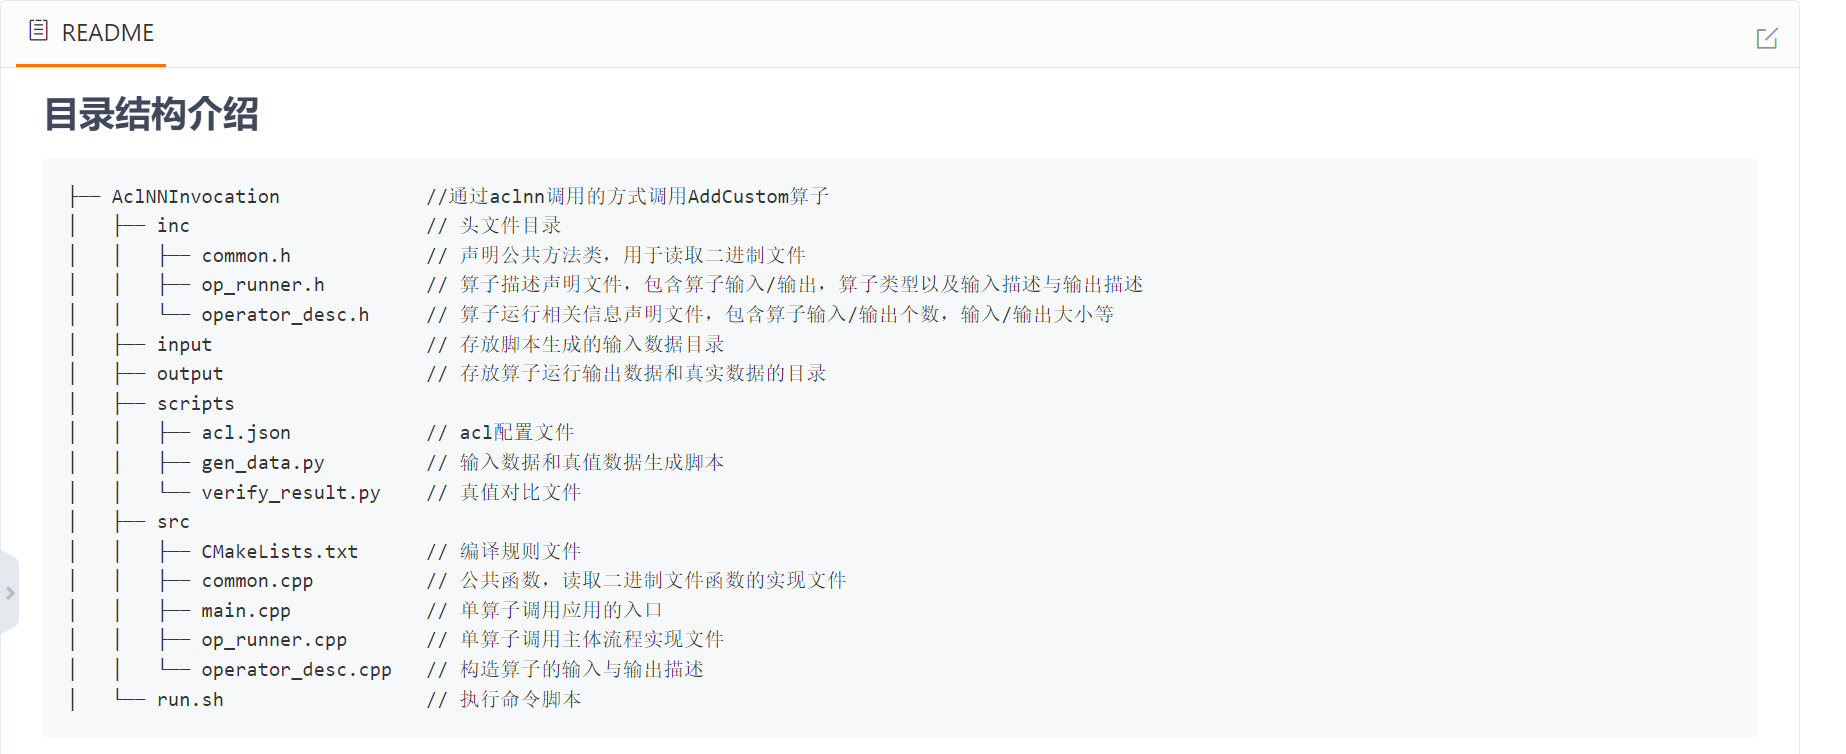
\includegraphics[width=1\linewidth]{screenshot001} % Adjust the width to 80% of the line width
		\caption{目录结构}
		\label{fig:screenshot001}
	\end{figure}
		\section{算子主机和设备端的工作}
	\subsection{主机侧}
	定义好有多少核,怎么切分数据,主要是完成把数据准备好,切分策略确定,送往设备侧运算\\
	用到的数据结构的详细解释(待补充)
	\begin{itemize}
		\item TilingContext:
		\item TilingData:
		\item context:
	\end{itemize}
	\subsection{设备侧}
	\begin{itemize}
	\item 分给每个核的大份数据分成能被核心一次性处理的n组tile
	\newpage		
		\lstinputlisting[language=C++,caption={add\_custom\_init}]{add_custom_init.cpp}
	\item 处理三步骤 CopyIn,Compute,CopyOut\\
	CopyIn:把数据片搬入设备\\
	Compute:负责设备内数据运算\\
	CopyOut:把运算结果搬到内存\\
	它们看似是得等前一步执行完才能到后一步,要等很长时间,实际上是指令的发送顺序,不用等命令执行完,这些指令被很快的按这个次序发送到设备的指令队列,在那里形成流水
	\item 队列中buffer num的个数对性能的影响:
	\begin{itemize}
		\item Q1: 怎么影响性能的?
		\item A1:待补充,没理清楚
	\end{itemize}
    \end{itemize}
\end{document}
